\section{Homographies}

\begin{frame}{\secname}
    ``The homograph is a mapping between two perspective images of a planar surface in a scene'' \cite{gledhill_panoramic_2003}
    \begin{figure}
        \centering
        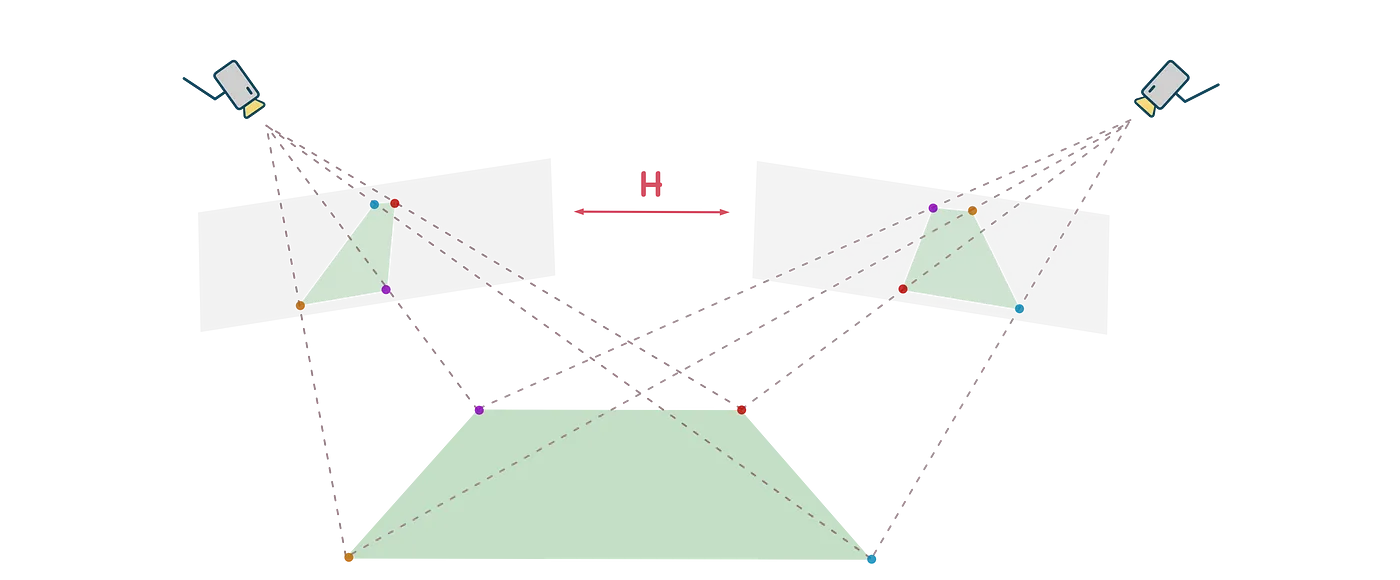
\includegraphics[width=\textwidth]{img/homog}
    \end{figure}
\end{frame}

\begin{frame}{\secname}
    An homography is just a matrix that convert some points into others.
    \begin{gather*}
        \lambda
        \begin{bmatrix}
            x' \\ y' \\ 1
        \end{bmatrix} = 
        \begin{bmatrix}
            H_{1,1} & H_{1,2} & H_{1,3} \\
            H_{2,1} & H_{2,2} & H_{2,3} \\
            H_{3,1} & H_{3,2} & H_{3,3}
        \end{bmatrix}
        \begin{bmatrix}
            x \\ y \\ 1
        \end{bmatrix}
    \end{gather*}    
\end{frame}


\begin{frame}{\secname}{Use case: How far was this shot?}
    By using homographies we can remove the perspective from an image, and after that we can measure in the image.
    \begin{figure}
        \subfloat{\includegraphics[width=0.5\textwidth]{img/puntoshomog_orig}}
        \subfloat{\includegraphics[width=0.4\textwidth]{img/puntoshomog_ref}}
    \end{figure}
\end{frame}

\begin{frame}{\secname}{Use case: How far was this shot?}
    By using homographies we can remove the perspective from an image. 
    \begin{figure}
        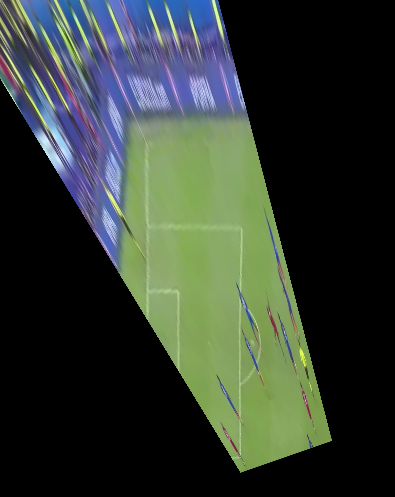
\includegraphics[width=0.5\textheight]{img/homog_eden}
    \end{figure}
\end{frame}

\begin{frame}{\secname}{Use case: How far was this shot?}
    We can establish measurements in the image.
    \begin{figure}
        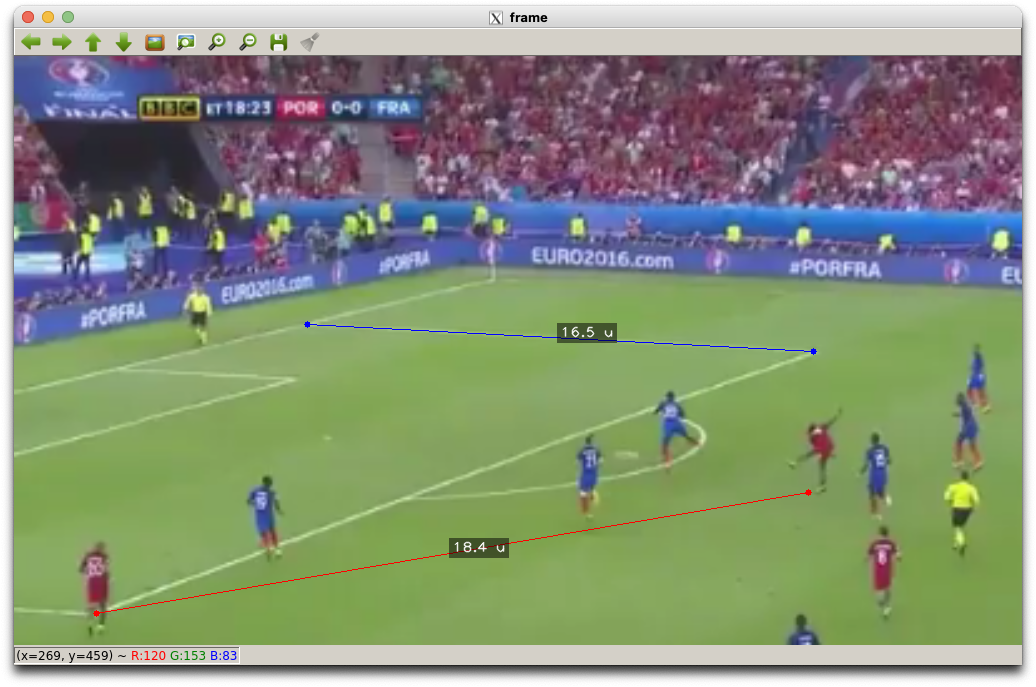
\includegraphics[width=0.7\textheight]{img/Medida_HomogOrig_Final}
    \end{figure}
\end{frame}

\begin{frame}{\secname}{Use case: How far was this shot?}
    Using trigonometry, as before, we can estimate the shot distance.
    \begin{figure}
        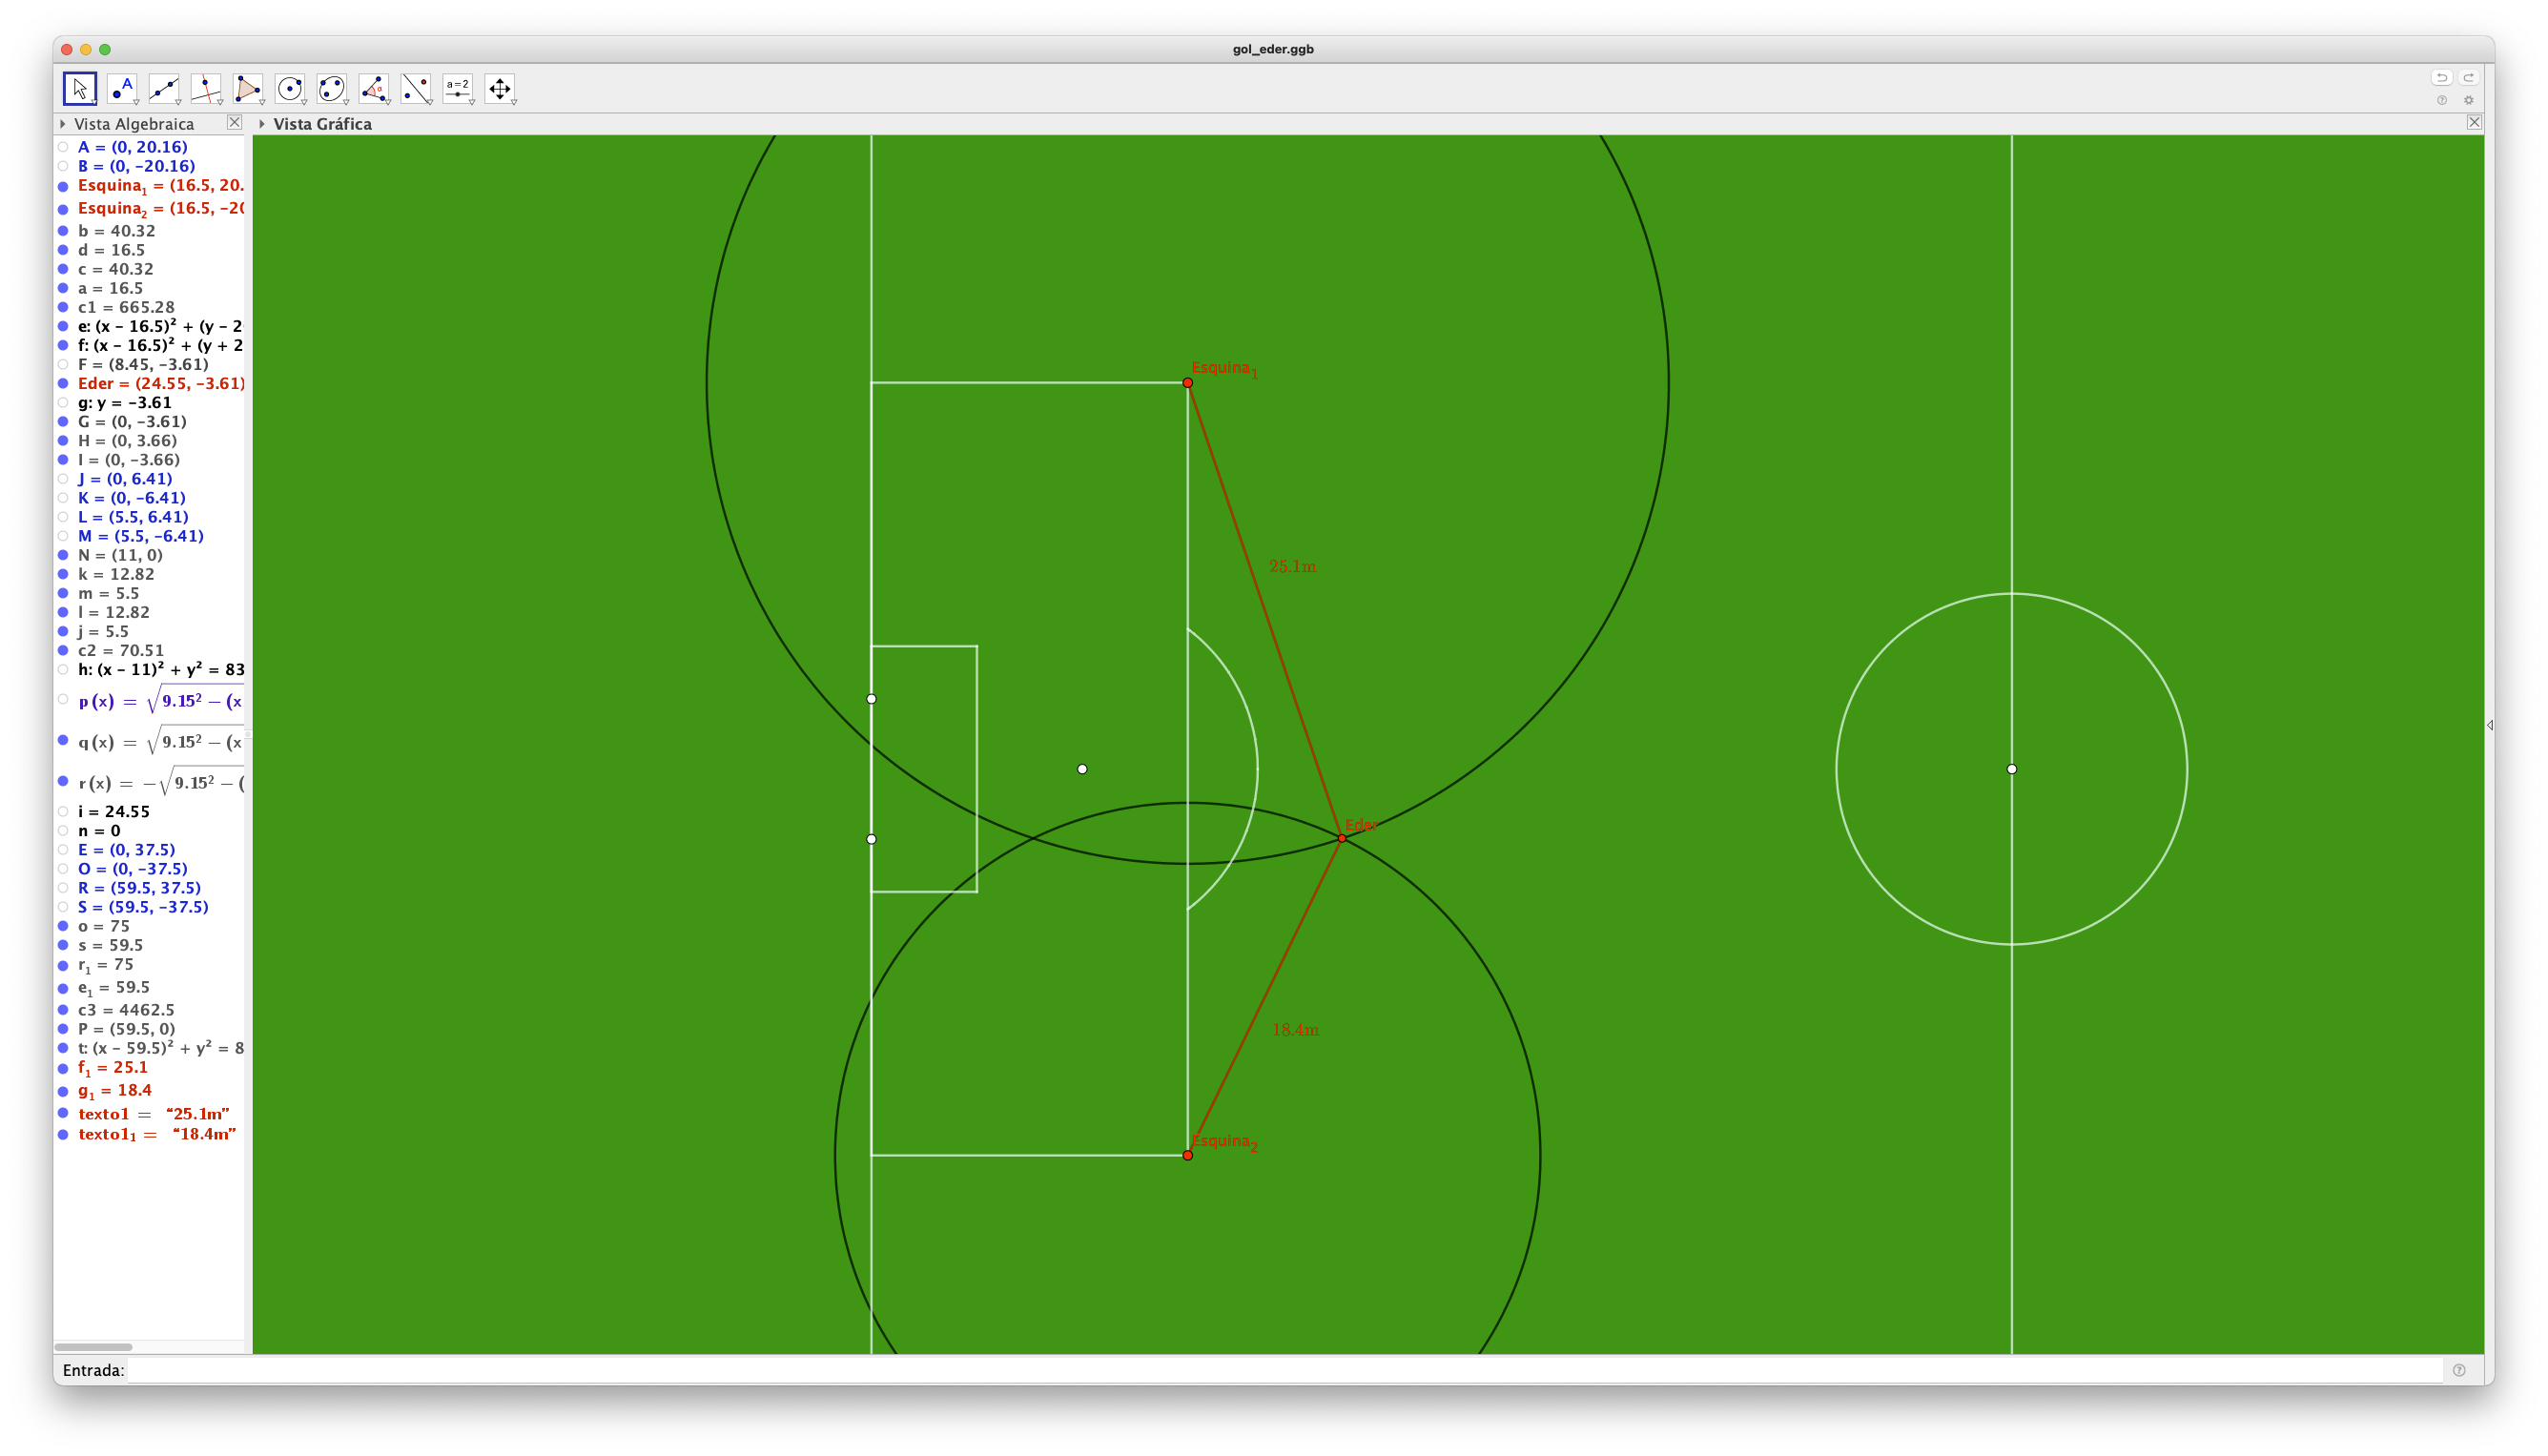
\includegraphics[width=\textwidth]{img/posicion-eder}
    \end{figure}
\end{frame}

